
\section{Results}
In this section, we present the results of the performance for pattern matching of the two graph databases: Neo4j and OrientDB. In ~\ref{setup}, we provide details of the machine used for the experiments and in ~\ref{result}, we present the results and discuss the optimization we did to run the pattern matching queries terminate faster.

\subsection{Experimental Setup}
\label{setup}

The machine we used for our experiment was large memory machine (256 GB): 2 socket Intel(R) Xeon(R) CPU E5-2650 @ 2.00GHz processors (32 cores). This machine was large enough to load IMDB graph ~\cite{IMDb96:online} in the memory.

\subsection{Loading IMDB data}
\subsubsection{ Neo4j}
We used neo4j LoadCSV tool~\cite{CSVImpor74:online} to load data into Neo4j. It took less than a minute (42 seconds) to load the data into Neo4j. After loading the database occupies 1.2GB of disk space.

\subsubsection{OrienDB}
We imported the data into OrientDB using OrienDB Importer~\cite{orientdb_importer} and it took 295 minutes to import the data. It occupies approximately 6GB of disk space.

\subsection{Query performance}
\label{result}
We obtained the results by running one pattern matching query on one database at a time to make sure that the query performance is not impacted due to other execution of other queries.

\subsubsection{Pattern 1-3}

We started with pattern matching query Pattern 1 on the Neo4j database and to our surprise, it took around 9 hours for the query to terminate. Hence, we optimized the query by running the query in the multiple threads at a time. As there were 32 cores on the machine and total of around 3.6 million person vertices (actors, actresses, and directors) to run the pattern matching query. Hence, we first use 20 threads for first 2 million and then 16 threads for remaining using a pool of threads. With each thread processing 100k vertices, the total time for Pattern 1 reduced to around 30 minutes for Neo4j. We did the same optimization for two other queries and for both graph databases.

\begin{comment}
\begin{table}[h!]
\resizebox{0.8\textwidth}{!}{%
%\captionof{table}{Neo4j:per thread execution time}
\begin{minipage}[b]{80mm}
\centering
\begin{tabular}{|c|c|c|c|} 
47

\hline
& Pattern 1 & Pattern 2 & Pattern 3 \\ 
\hline
Thread	0	&  977.89	&	836.84 &	925.05   \\ 
 \hline 
Thread	1	&  969.99	&	846.65 &	919.52   \\ 
 \hline 
Thread	2	&  909.21	&	853.76 &	914.13   \\ 
 \hline 
Thread	3	&  997.76	&	856.53 &	906.03   \\ 
 \hline 
Thread	4	&  988.03	&	853.99 &	914.15   \\ 
 \hline 
Thread	5	&  961.67	&	840.02 &	916.63   \\ 
 \hline 
Thread	6	&  989.58	&	867.04 &	924.72   \\ 
 \hline 
Thread	7	&  945.33	&	856.65 &	920.63   \\ 
 \hline 
Thread	8	&  989.86	&	871.52 &	923.34   \\ 
 \hline 
Thread	9	&  980.54	&	864.57 &	915.12   \\ 
 \hline 
Thread	10	&  987.06	&	864.91 &	926.87   \\ 
 \hline 
Thread	11	&  989.20	&	853.66 &	918.73   \\ 
 \hline 
Thread	12	&  986.01	&	858.76 &	919.60   \\ 
 \hline 
Thread	13	&  986.55	&	858.80 &	922.03   \\ 
 \hline 
Thread	14	&  983.65	&	855.88 &	921.39   \\ 
 \hline 
Thread	15	&  988.05	&	859.70 &	923.25   \\ 
 \hline 
Thread	16	&  979.21	&	855.41 &	922.93   \\ 
 \hline 
Thread	17	&  979.74	&	858.52 &	922.98   \\ 
 \hline 
Thread	18	&  983.90	&	853.14 &	920.50   \\ 
 \hline 
Thread	19	&  980.60	&	857.86 &	918.19   \\ 
 \hline 
Thread	20	&  758.00	&	698.05 &	736.53   \\ 
 \hline 
Thread	21	&  745.77	&	705.25 &	739.87   \\ 
 \hline 
Thread	22	&  742.99	&	704.31 &	736.87   \\ 
 \hline 
Thread	23	&  746.04	&	684.15 &	746.56   \\ 
 \hline 
Thread	24	&  776.15	&	684.06 &	736.88   \\ 
 \hline 
Thread	25	&  772.49	&	697.14 &	737.96   \\ 
 \hline 
Thread	26	&  771.59	&	701.06 &	735.97   \\ 
 \hline 
Thread	27	&  773.59	&	683.95 &	741.41   \\ 
 \hline 
Thread	28	&  771.33	&	683.18 &	739.43   \\ 
 \hline 
Thread	29	&  773.60	&	700.56 &	742.52   \\ 
 \hline 
Thread	30	&  771.13	&	690.38 &	742.13   \\ 
 \hline 
Thread	31	&  770.64	&	681.84 &	739.73   \\ 
 \hline 
Thread	32	&  736.51	&	676.41 &	741.01   \\ 
 \hline 
Thread	33	&  677.96	&	668.71 &	733.49   \\ 
 \hline 
Thread	34	&  678.34	&	668.84 &	736.02   \\ 
 \hline 
Thread	35	&  676.23	&	666.83 &	736.76   \\ 
 \hline 
\end{tabular}
\caption{Neo4j: per thread execution time}
\label{table:neo4j}
\end{minipage}

\quad
\begin{minipage}[b]{80mm}
\centering
\begin{tabular}{|c|c|c|c|}
\hline
& Pattern 1 & Pattern 2 & Pattern 3 \\ 
\hline
Thread	0	&  2431.68  &	2225.29   & 	2015.88  \\ 
 \hline 
Thread	1	&  2391.48  &	2102.63   & 	2017.00  \\ 
 \hline 
Thread	2	&  2301.36  &	2127.60   & 	2012.43  \\ 
 \hline 
Thread	3	&  2379.92  &	2156.31   & 	2068.56  \\ 
 \hline 
Thread	4	&  2278.00  &	2129.00   & 	2013.33  \\ 
 \hline 
Thread	5	&  2288.26  &	2129.44   & 	2010.54  \\ 
 \hline 
Thread	6	&  2329.51  &	2147.03   & 	2078.90  \\ 
 \hline 
Thread	7	&  2292.64  &	2076.83   & 	2005.99  \\ 
 \hline 
Thread	8	&  2300.49  &	2143.34   & 	2053.73  \\ 
 \hline 
Thread	9	&  2310.48  &	2115.65   & 	2085.95  \\ 
 \hline 
Thread	10	&  2282.12  &	2237.32   & 	2016.41  \\ 
 \hline 
Thread	11	&  2280.59  &	2139.30   & 	2022.68  \\ 
 \hline 
Thread	12	&  2304.19  &	2222.45   & 	2021.72  \\ 
 \hline 
Thread	13	&  2299.62  &	2129.33   & 	2011.10  \\ 
 \hline 
Thread	14	&  2309.20  &	2098.21   & 	2053.04  \\ 
 \hline 
Thread	15	&  2310.07  &	2136.47   & 	1996.36  \\ 
 \hline 
Thread	16	&  2367.08  &	2144.35   & 	2021.97  \\ 
 \hline 
Thread	17	&  2308.65  &	2242.05   & 	2016.55  \\ 
 \hline 
Thread	18	&  2377.75  &	2225.02   & 	2031.90  \\ 
 \hline 
Thread	19	&  2299.53  &	2091.73   & 	2025.14  \\ 
 \hline 
Thread	20	&  1347.48  &	1160.90   & 	1071.00  \\ 
 \hline 
Thread	21	&  1343.23  &	1150.95   & 	1054.96  \\ 
 \hline 
Thread	22	&  1334.77  &	1157.36   & 	1104.03  \\ 
 \hline 
Thread	23	&  1350.81  &	1160.95   & 	1111.09  \\ 
 \hline 
Thread	24	&  1349.01  &	1167.03   & 	1104.19  \\ 
 \hline 
Thread	25	&  1355.92  &	1171.55   & 	1104.72  \\ 
 \hline 
Thread	26	&  1422.85  &	1164.85   & 	1108.75  \\ 
 \hline 
Thread	27	&  1349.25  &	1162.60   & 	1124.82  \\ 
 \hline 
Thread	28	&  1360.41  &	1184.17   & 	1086.14  \\ 
 \hline 
Thread	29	&  1351.56  &	1160.24   & 	1087.87  \\ 
 \hline 
Thread	30	&  1415.79  &	1157.77   & 	1106.59  \\ 
 \hline 
Thread	31	&  1349.18  &	1161.95   & 	1112.36  \\ 
 \hline 
Thread	32	&  1307.40  &	1129.19   & 	1104.93  \\ 
 \hline 
Thread	33	&  1148.93  &	1036.64   & 	1066.42  \\ 
 \hline 
Thread	34	&  1121.97  &	1023.64   & 	1051.95  \\ 
 \hline 
Thread	35	&  1087.44  &	959.72    & 	1059.18  \\ 
 \hline
\end{tabular}
\caption{OrientDB: per thread execution time}
\label{table:orient}
\end{minipage}
}%resizebox
\label{table:orientdb-per thread}
\end{table}

\end{comment}


\begin{table}[h!]
\resizebox{0.7\textwidth}{!}{%
%\captionof{table}{Neo4j:per thread execution time}
\begin{minipage}[b]{80mm}
\centering
\begin{tabular}{|c|c|c|c|c|c|}
\hline
 & Time (in hrs) & CPU (avg/max) & Memory (avg) & Pattern instances\\
\hline
Pattern	1 	& 0.48  &    320\%/400\%	&   1.2 \% & 3590 \\
Pattern	2 	& 0.43  &    250\%/363\%	&   1.3\%	&  8437 \\
Pattern	3 	& 0.46  &    175\%/300\%	&	1.4\%  & 1806\\
Pattern	4 	& 30.77 &    163\%/2298\%	&	1.3\%  & 4812  \\
Pattern	5 	& 11.77 &    163\%/2298\%	&	1.3\%  & 263 \\
Pattern	6 	& 18.38 &    163\%/2298\%	&	1.3\%  & 9 \\

\hline
\end{tabular}
\caption{ Performance data for Neo4j}
\label{table:neo4j}
\end{minipage}
}%resizebox
\label{table:orientdb-per thread}
\end{table}

\begin{table}[htb!]
\resizebox{0.7\textwidth}{!}{%
\begin{minipage}[b]{80mm}
\centering
\begin{tabular}{|c|c|c|c|c|c|}
\hline
 & Time (in hrs) & CPU (avg/max) & Memory (avg) & Pattern instances\\
\hline
Pattern	1 	& 1.03  &    964\%/1400\%	&   27.34 \% & 3590 \\
Pattern	2 	& 0.92  &    941\%/1319\%	&   26.88\%	&  8437 \\
Pattern	3 	& 0.87  &    548\%/1260\%	&	27.25\%  & 1806\\
Pattern	4 	& 65.50 &    86.7\%/2298\%	&	11.3\%  & 4812  \\
Pattern	5 	& 20.19 &    86.7\%/2298\%	&	11.3\%  & 263 \\
Pattern	6 	& 20.21 &    86.7\%/2298\%	&	11.3\%  & 9 \\

\hline
\end{tabular}
\caption{ Performance data for OrienDB}
\label{table:orient}
\end{minipage}
}%resizebox
\end{table}


\begin{figure}[h!]

	\resizebox{.8\linewidth}{!}{
		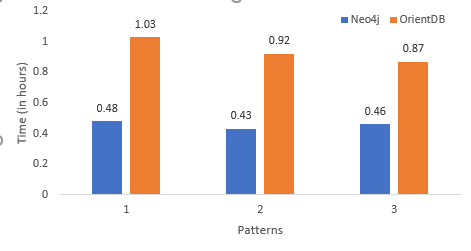
\includegraphics[width=0.8\linewidth]{Images/comp1.png}
	}
	\caption{Graph databases: Performance comparison for patterns 1-3}
	\label{fig:1-3}
	\centering
\end{figure}

\begin{figure}[h!]

	\resizebox{.8\linewidth}{!}{
		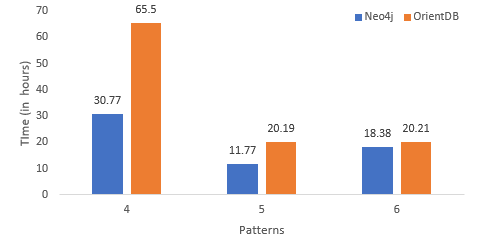
\includegraphics[width=0.8\linewidth]{Images/comp2.png}
	}
	\caption{Graph databases: Performance comparison for patterns 4-6}
	\label{fig:4-6}
	\centering
\end{figure}


\subsubsection{Pattern 4-6}

Compared to patterns 1-3, the patterns 4-6 are more intensive. We ran the pattern-matching queries for patterns 4-6 one at a time, we observed that execution did not complete even in 25 days. So, we decided to run the queries on the subset of movies nodes (50k) in the graph rather than all the movies nodes (1.3m). 

The time taken, CPU and memory utilization and total vertices that particapted in each query by for Neo4j and OrientDB are shown in the Tables~\ref{table:neo4j} and ~\ref{table:orient} respectively.

We can see from the Figures~\ref{fig:1-3} and ~\ref{fig:4-6} that the Neo4j's performance is better (1.1x - 2.1) than OrientDB.

\subsection{Expressibility of queries in Gremlin}

Gremlin is a path-oriented language~\cite{Chapter635:online}. It is easy to implement queries that follow a path. For example, it is easy to get a movie and each actor, actress, and director worked in that movie because all this nodes are in one path and query starts with one type vertices. 

Not all queries have single paths, for example query 3 starts with three entry points actor, actress, and director and hard to write in gremlin.

We in this project use python to overcome this drawback in gremlin. 

\section{Conclusions}
From the experimental results, it is clear that the Neo4j performs better than OrientDB (1.1x - 2.1x). CPU utilization is more in OrientDB  for patterns 1-3 whereas more in patterns 4-6. The memory utilization in OrientDB exceeded that in Neo4j for all the patterns.

Caching did not have much effects on the queries that were run subsequently i.e. we got performance improvement by 0.007\% in case of the queries.

We also found that there were various versions mismatch issues between the databases, Tinkerpop, and dependent libraries for which we had to do a lot of trial and error to make the experiment work.

\section{Future Work}
OrientDB and Neo4j both claim to be a native graph database. OrientDB supports multi-models such as the key-value store, a document store, and graph database. as such it's a graph database with nodes as a document. Neo4j only allows the graph to be stored as a property graph. From the results we got, it definitely seems that Neo4j is more optimized when compared to orientDB. Study of optimizations that contributed to the superior performance of Neo4j will be future work for this project.